\section{Wikiaves x SpeciesLink}

\hrulefill



\hrulefill


\begin{resposta}
Para relacionar as quantidades de registros e espécies dos bancos de dados, há de se dispor dos dados de forma diferente da apresentada anteriormente. A tabela (matriz) a seguir traz os valores de $p$ e $r$, respectivamente, acima e a abaixo da diagonal principal.
\end{resposta}

\newpage

\subsection{Registros}

\begin{figure}[h!]
\centering
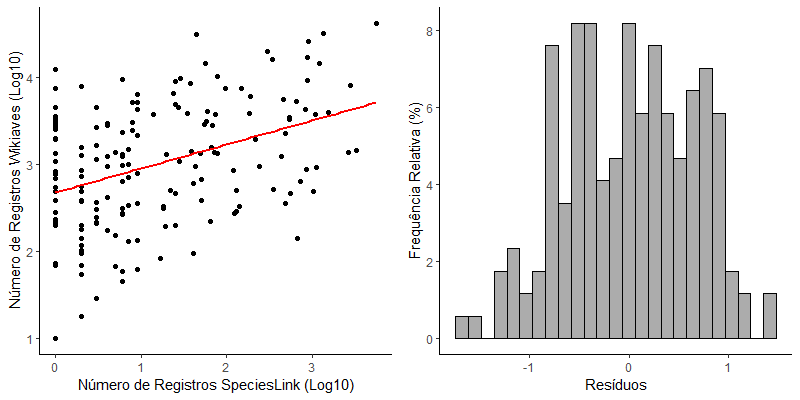
\includegraphics[width = 12cm]{Imagens/G11.png}
\\{\scriptsize  Figura 19: Relação linear entre o número de registros (Log10) nos bancos de dados SLI e WAV2 pareados por X municípios redundantes e respectiva distribuição de resíduos (direita, em unidades de desvio-padrão). Outliers bivariados foram excluídos. n = 171, r2 = 0,1588, P < 0,0001 .}
\end{figure}

\begin{resposta}
Pelos valores de $p$ expostos na tabela, os resultados experimentais possuem relação. Ao parear o log da quantidade de registros dos dois bancos de dados, obtém-se um coeficiente de correlação linear de 0,41. Este valor não é alto em comparação a outros que já obtidos, porém, o gráfico indica um crescimento linear.

Ao excluir os pares ordenados que geram resíduos discrepantes, há um aumento do valor de $p$ para $6,74*10^{-8}$ e uma diminuição de $r$ para $0,40$. Indicando que esses pares tem influência sob a curva.
\end{resposta}




\subsection{Espécies}

\begin{figure}[h!]
\centering
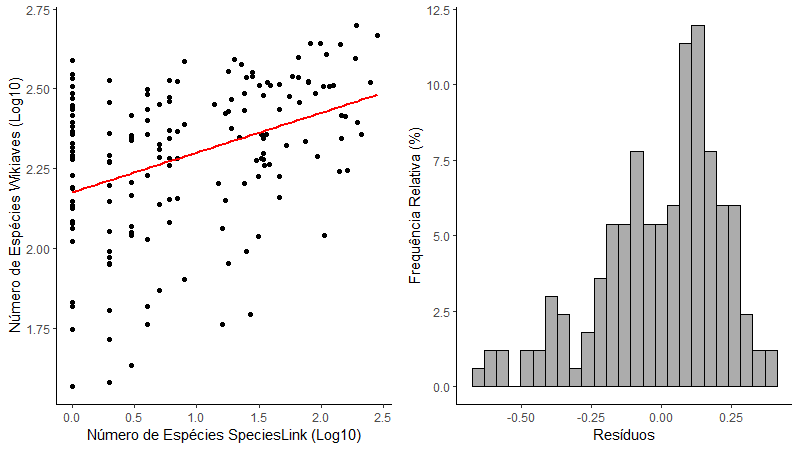
\includegraphics[width = 12cm]{Imagens/G12.png}
\\{\scriptsize Figura 20: Relação linear entre o número de espécies (Log10) nos bancos de dados SLI e WAV2 pareados por X municípios redundantes e respectiva distribuição de resíduos (direita, em unidades de desvio-padrão). Outliers bivariados foram excluídos. n = 167 , r2 = 0,1523 , P < 0,0001 .}
\end{figure}

\begin{resposta}
Novamente, pelo valor $p$, é possível que haja relação entre os dados. O valor de $r$ é muito parecido com o anterior: $0,40$. Ou seja, a correlação linear é ligeiramente menor. Não obstante, no gráfico abaixo, nota-se que há uma correlação linear. 

\end{resposta}

\subsection {Registros x Espécies}

\begin{figure}[h!]
\centering
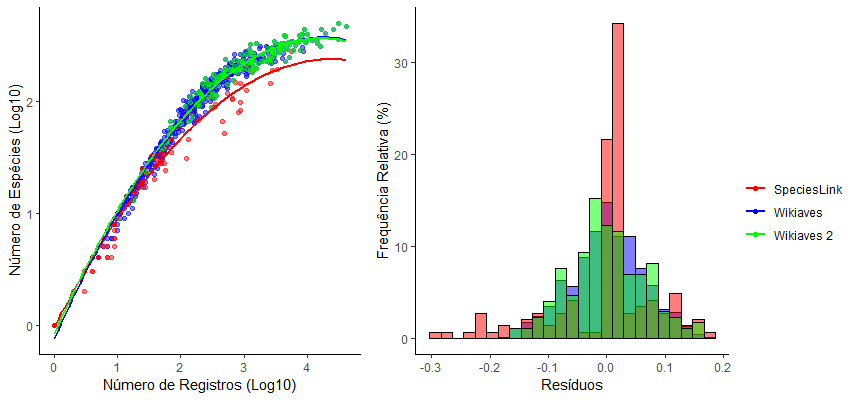
\includegraphics[width = 15cm]{Imagens/G13.png}
\\{\scriptsize Figura 21: Relação quadrática entre o número de espécies e o número de registros (ambos em Log10) nos bancos de dados WAV, SLI e WAV2 pareados por município e respectiva distribuição de resíduos (direita, em unidades de desvio-padrão). Outliers bivariados foram excluídos. n = 620, r2 = 0,9875, P < 0,0001 no Wikiaves. n = 143, r2 = 0,9867, P < 0,0001 no Wikiaves. n = 171, r2 = 0,9647, P < 0,0001 no Wikiaves 2.}
\label{Figura 20}
\end{figure}

\begin{resposta}
Até o momento, os valores de $r$ são os maiores encontrados: para o Wikiaves $0,91$ e para o SpeciesLink $0,94$. Porém, o gráfico traz fortes indicativos de que a correlação não é linear.

Portanto, ao assumir que a correlação não é linear obtemos aproximações mais exatas para as curvas, nestas os valores de $r^2$ são de $0,9604$ no Wikiaves e $0,9067$ no SpeciesLink, isto é, os valores próximos de 1 indicam que há forte correlação nas aproximações abaixo.

É possível, ainda, otimizar estes valores ao retirar os resíduos discrepantes. No Wikiaves, há um leve aumento de $r^2$ para $0,9647$.


\end{resposta}